\documentclass[12pt, a4paper] {ncc}
\usepackage[utf8] {inputenc}
\usepackage[T2A]{fontenc}
\usepackage[english, russian] {babel}
\usepackage[usenames,dvipsnames]{xcolor}
\usepackage{listings,a4wide,longtable,amsmath,amsfonts,graphicx}
\usepackage{indentfirst}
\usepackage{bytefield}
\usepackage{multirow}
\usepackage{float}
\usepackage{caption}
\usepackage{subcaption}
\captionsetup{compatibility=false}
\usepackage{tabularx}

\usepackage[left=2cm,right=2cm,top=2cm,bottom=2cm,bindingoffset=0cm]{geometry}

\begin{document}
\setcounter{figure}{0}
\frenchspacing
\pagestyle{empty}
\begin{center}
                            Университет ИТМО    \\
                        Кафедра вычислительной техники

\vspace{\stretch{2}}
                    Комьютерная графика
\end{center}
\vspace{\stretch{2}}
\begin{center}
                            Лабораторная работа
\end{center}
\vspace{\stretch{3}}
\begin{flushright}
                                    Студент:\\
                                    {\it Куклина Мария,}\\
                                    Преподаватель: \\
                                    {\it Королёва Ю.А..}
\end{flushright}
\vspace{\stretch{4}}
\begin{center}
                             Санкт-Петербург, 2017
\end{center}
\newpage

\section{Задание}
	Разработать ПО, которое отображает сцену из нескольких сложных объектов с использовнием
	OpenGl. Сцента должна содержать несколько источников света, иметь прозрачные объекты и
	провильно рассчитывать тени для прозрачных и непрозрачных объектов (без учёта свойств
	их материалов).

\section{Карта теней}
	\subsection{Алгоритм}
		Идея алгоритма получения теней состоит в использовании буфер глубины для решения,
		находится ли обрабатываемая точка в тени.
	
		Для этого сцена рендерится относительно источника света в буфер глубины. Полученные
		значения глубины используются при определении цвета точки: если длина луча от источника
		света до точки больше, чем значение глубины на пути луча, то точка находится в тени.

	\subsection{Результат теней от двух источников света}

		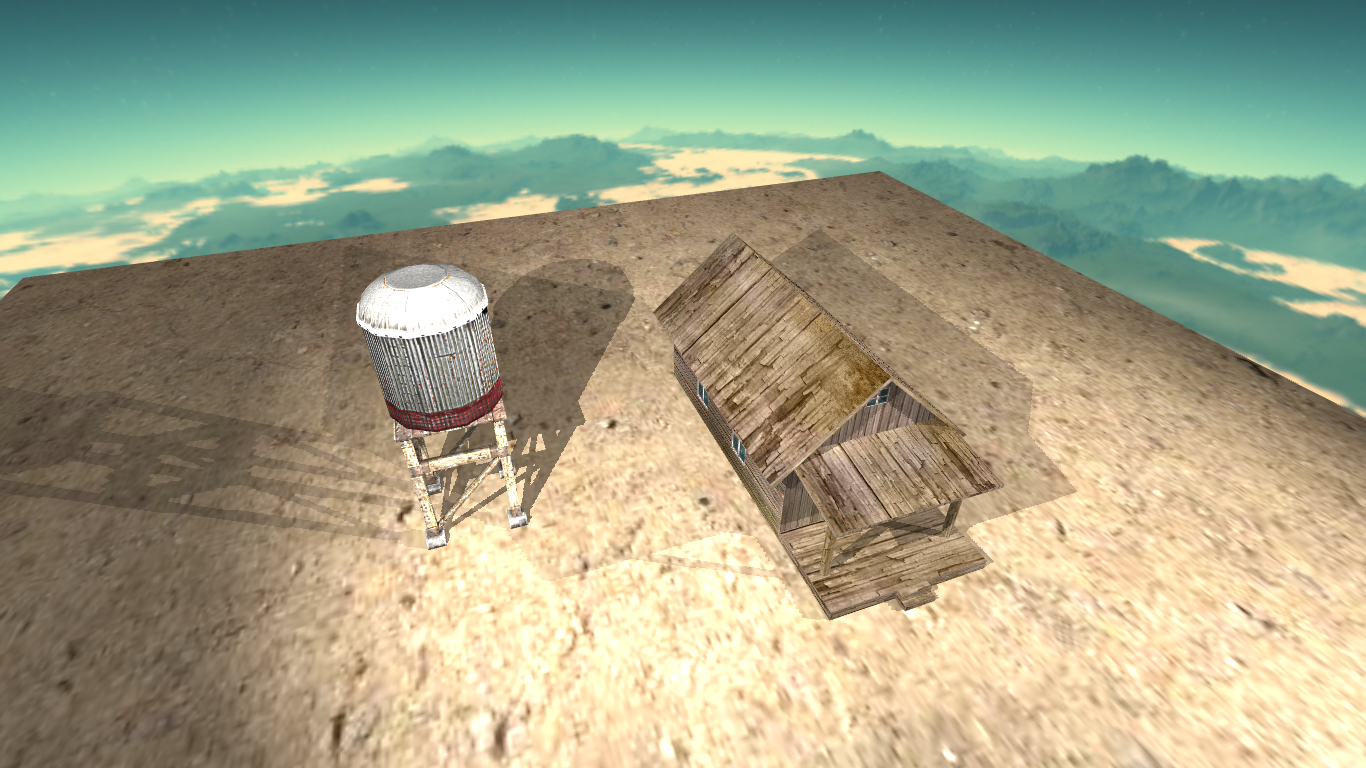
\includegraphics[scale=0.3]{./scene.png}

\section{Прозрачность}

	Для того, чтобы отображать прозрачные предметы, используется функцию блендинга. Во время
	стадии блендинга инвертированный $\alpha$-канал исходного фрагмента
	умножается на компоненты цвета, что делает весь объект тем светлее, чем меньше $\alpha$.
	Однако для создания эффектра прозрачности так же нужно отключить проверку глубины, чтобы
	отрисовывались все полигоны прозрачного объекта.

	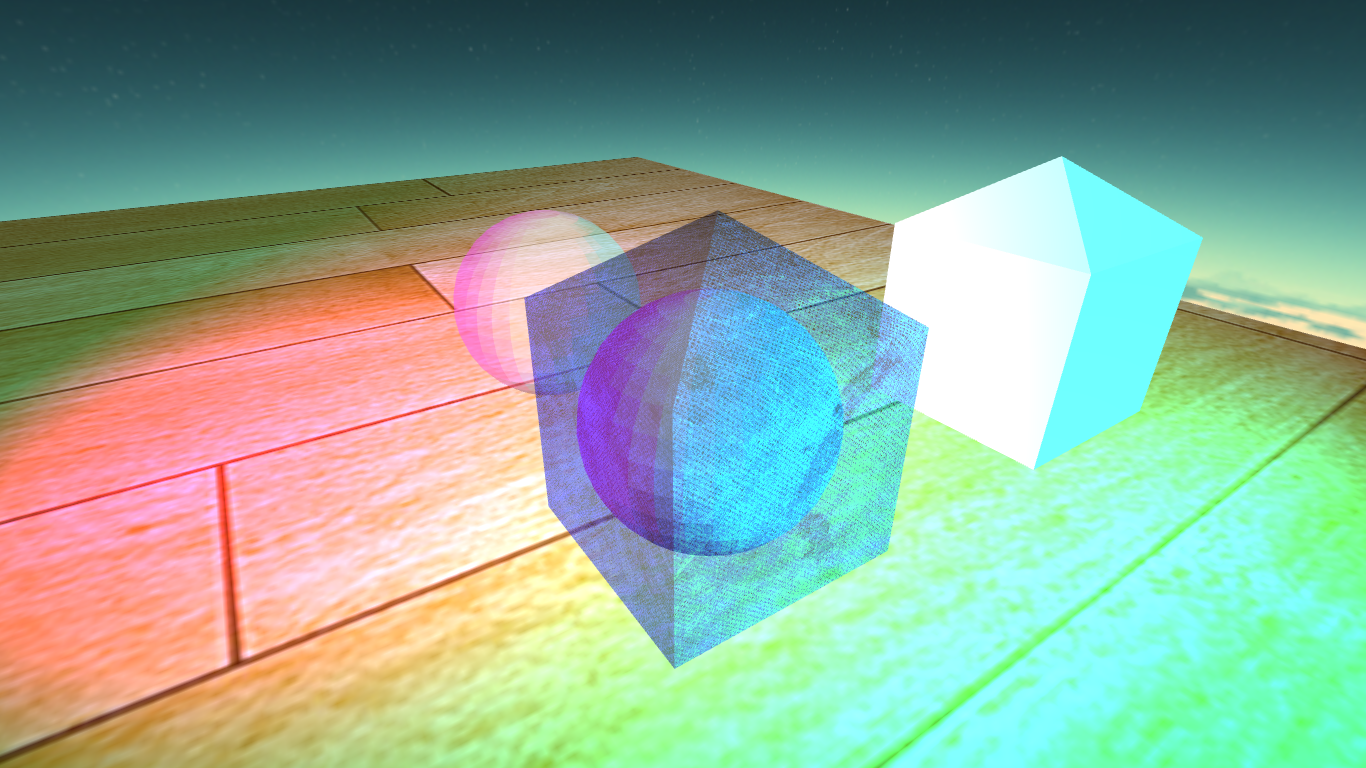
\includegraphics[scale=0.3]{./scene_transp.png}

	Метод карты теней не учитывает степень прозрачности объекта, из-за чего, к примеру,
	в случае, когда непрозрачный объект вложен в прозрачный, тень либо от только непрозрачного 
	объекта, либо от внешнего прозрачного объекта, в зависимости от того, для чего производится
	расчёт тени. Однако прозрачные объекты задерживают не весь свет, а только
	его часть, в зависимости от степени прозрачности, и пропускают тени от других объектов.
	Метод карты теней нам не позволяет делать подобные рассчёты.

	\subsection{Алгоритм}
		Для вычисления теней от прозрачных объектов был разработан несложный алгоритм,
		основанный на методы карты теней.
		\begin{enumerate}
			\item Строим сцену из объектов и расскрашиваем их таким образом, что прозрачным объектам
			   выделяется один канал цвета, а непрозрачным -- другой (или вовсе не выделяется, что
			   соответствует чёрному цвету). Из-за того, что $\alpha$-канал у прозрачных объектов не
			   нулевой результирующий цвет этих объектов будет соответствовать степени прозрачности
			   объекта, а пересечению прозрачных объектов будет соответствовать суммарное вложение
			   интенсивностей от каждого объекта. Таким образом, строится то, что мы в данной работе
			   называем \textit{картой прозрачности}.
			\item Про рендере карты теней из сцены исключаются прозрачные объекты, чтобы иметь возможность
			   расчитать тени от непрозрачных объектов.
			\item На стадии финальной отрисовки объектов принимаем решение о наличие тени и степени затенённости
			   на основе карты теней и карты прозрачности: если длина луча от источника света до точки, больше
			   чем глубина этого луча, то объект находится в тени от непрозрачного объекта, в ином случае
			   используем интенсивность канала цвета для этого луча из карты прозрачности (если интенсивность 0,
			   то ничего не преграждает путь лучу, в ином случае на пути до точки задерживается количество
			   света, равное интенсивности, поэтому коэффициент затенения высчитывается как $1 - \text{интенсивность}$.
		\end{enumerate}

		\begin{figure}[ht]
        	
\includegraphics[scale=0.3]{./scene_transp_map.png}
			\caption{Карта прозрачности от одного источника света}
		\end{figure}

\newpage
	\subsection{Результат}
	
		\begin{figure}[ht]
        	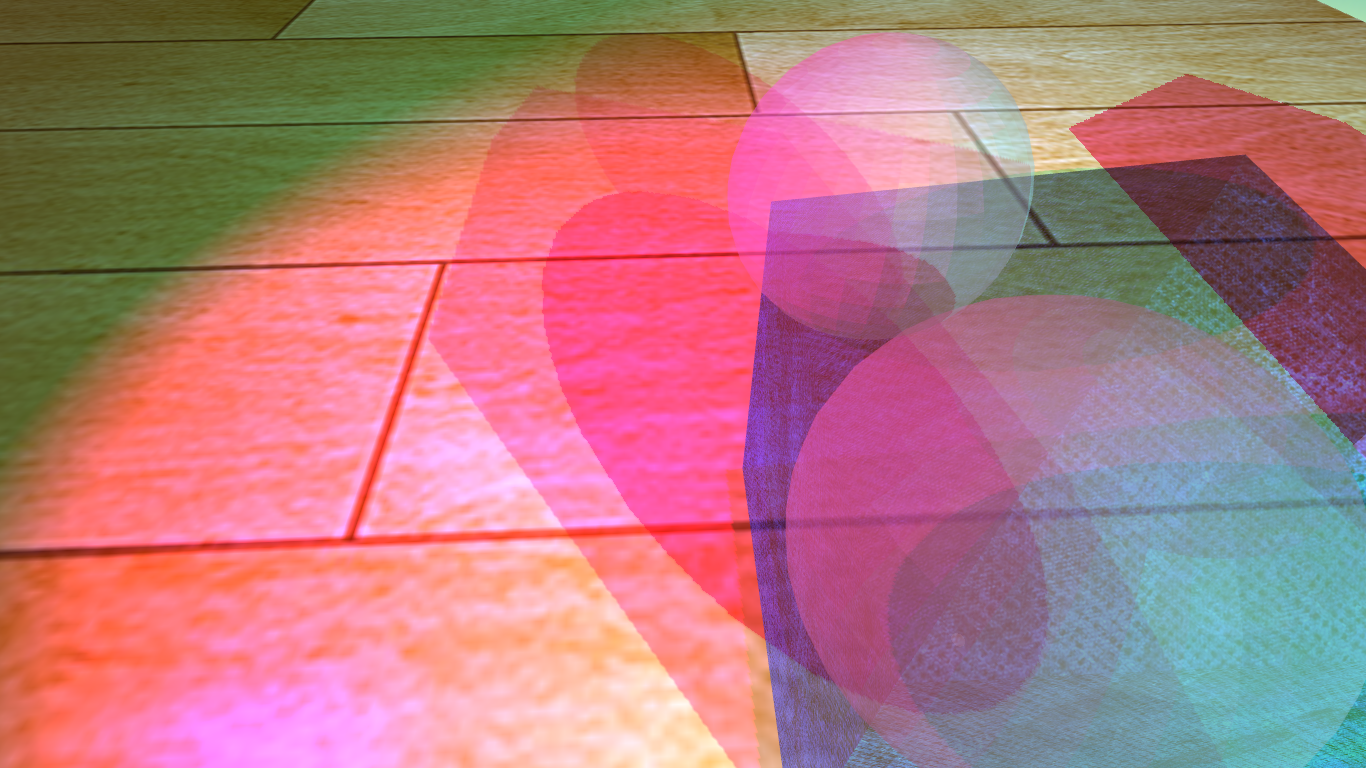
\includegraphics[scale=0.3]{./shadow_tr1.png}
    		\caption{Тени от нескольких прозрачных объектов}
		\end{figure}

		\begin{figure}[ht]
        	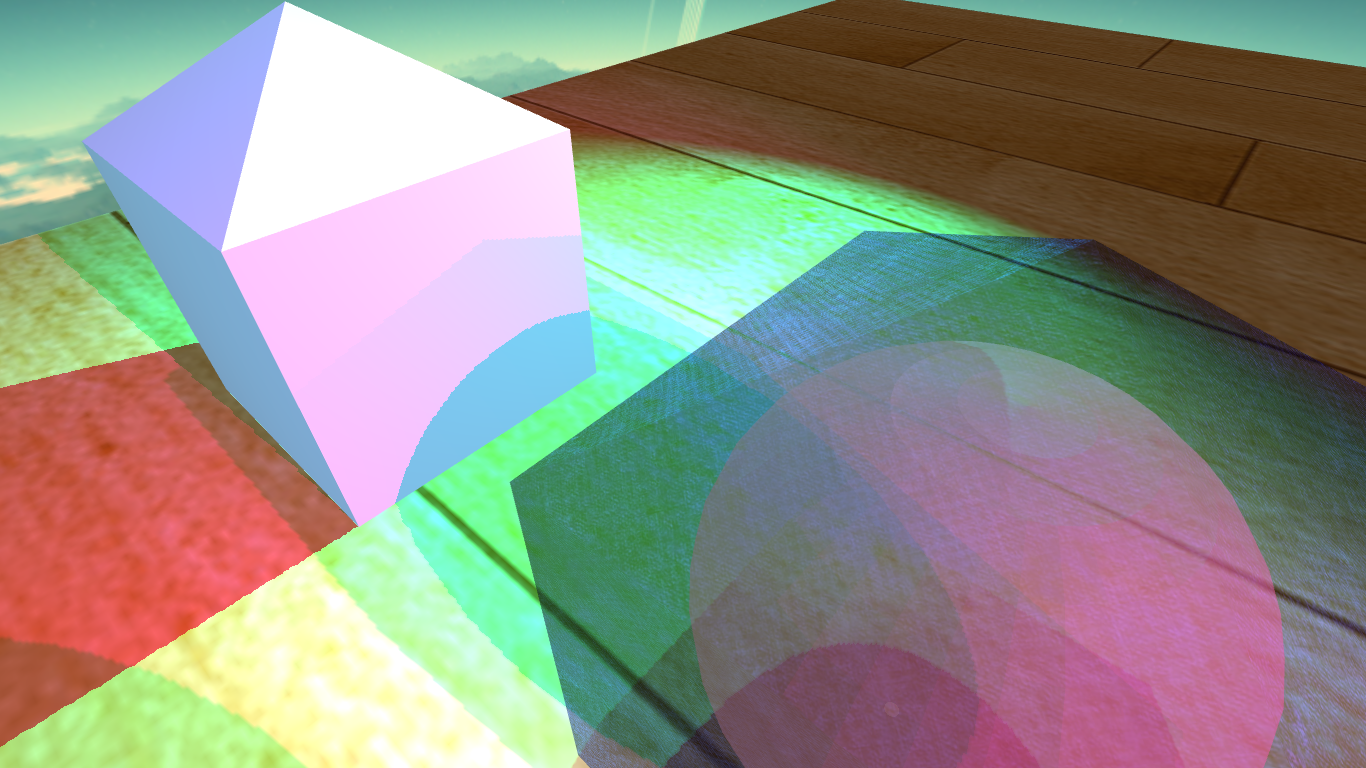
\includegraphics[scale=0.3]{./shadow_tr2.png}
    		\caption{Тени на напрозрачных объектах}
		\end{figure}
\end{document}
